\chapter{PPO mit bedingtem Aktionsraum}
\label{ch:ppo_bedingt}

Dieses Kapitel widmet sich der Anpassung des PPO-Algorithmus an die spezifische Struktur des hybriden und bedingten Aktionsraums. Eine zentrale Herausforderung besteht hierbei in der hierarchischen Abhängigkeit zwischen den Teilaktionen, welche von Standard-Implementierungen oft nicht korrekt abgebildet wird.
\vspace{\baselineskip}

Die verwendete sb3-Plus Bibliothek geht davon aus, dass alle Komponenten eines Aktionsvektors unabhängig voneinander gewählt werden können. Dies führt dazu, dass das Netzwerk auch dann versucht, einen optimalen Wert für die kontinuierliche Lenkaktion zu lernen, wenn der Agent sich entscheidet, gar nicht zu lenken (z.\,B. bei der Wahl von \emph{Noop} oder \emph{Direct Route}). In solchen Fällen ist der ausgegebene Lenkwert jedoch für die Umgebung bedeutungslos.
Ohne Anpassung würde der Algorithmus dennoch Gradienten für diese inaktiven Komponenten berechnen und das Netzwerk entsprechend aktualisieren. Dies verschwendet nicht nur Trainingskapazität, sondern kann den Lernprozess stören, da das Netzwerk versucht, Zusammenhänge zu lernen, wo keine sind. Im Folgenden wird eine Methode vorgestellt, die diese Abhängigkeiten berücksichtigt und sicherstellt, dass der Optimierungsschritt nur auf tatsächlich relevanten Aktionen basiert.
\vspace{\baselineskip}

\section{Verwandte Arbeiten und Abgrenzung}

Die Problematik gemischter Aktionsräume wird in der Literatur oft als \textit{Parameterized Action Space} bezeichnet. Masson et al. \cite{masson2016reinforcement} nutzen hierfür Q-Learning-Verfahren. Dabei gehen sie davon aus, dass zu jeder diskreten Aktion immer ein passender kontinuierlicher Parameter gehört, der mitgelernt werden muss.
Im vorliegenden Szenario erfordern Aktionen wie \emph{Noop} hingegen keinen Parameter. Der hier vorgestellte Ansatz verzichtet daher auf die Optimierung dieser irrelevanten Ausgabegrößen. Durch den Einsatz von Gradient-Gating wird sichergestellt, dass die entsprechenden Parameter vom Trainingsprozess ausgeschlossen werden, sofern sie für die getroffene diskrete Entscheidung keine Relevanz besitzen.
\vspace{\baselineskip}

Ein weiterer verwandter Ansatz ist das \emph{Invalid Action Masking} \cite{invalid_Action_Masking}. Dort kommt ein zustandsabhängiges Gating zum Einsatz, um ungültige Aktionen bereits während der Rollout\hyp{}Phase zu maskieren. Für das hier vorliegende Problem lässt sich dieser Ansatz jedoch nicht direkt übertragen. Die Relevanz der kontinuierlichen Aktion hängt nicht allein vom Zustand ab, sondern primär von der im selben Zeitschritt erst noch zu wählenden diskreten Aktion. Da diese Entscheidung zum Zeitpunkt einer potenziellen Maskierung noch nicht feststeht, ist ein präemptives Gating ausgeschlossen.

\section{Theoretische Fundierung der Anpassungen}

Ein Blick auf die mathematischen Grundlagen verdeutlicht, warum die Standard\hyp{}Implementierung hier unzureichend ist. Die ursprüngliche Implementierung geht davon aus, dass die logarithmischen Wahrscheinlichkeiten der Teilaktionen einfach addiert werden können. Wegen der Rechenregel $\log(p_1) + \log(p_2) = \log(p_1 \cdot p_2)$ entspricht dies einer Multiplikation der eigentlichen Wahrscheinlichkeiten. Diese Multiplikation setzt jedoch voraus, dass die Ereignisse unabhängig voneinander sind – eine Annahme, die in diesem Szenario verletzt ist, da die Relevanz der kontinuierlichen Aktion direkt von der diskreten Entscheidung abhängt.
\vspace{\baselineskip}

Um diese Abhängigkeit korrekt abzubilden, nutzt die Implementierung (siehe Abschnitt \ref{sc:ppo_anpassung}) eine \glqq Null-Maskierung\grqq{}. Dabei wird der Log\hyp{}Wahrscheinlichkeitswert einer irrelevanten Aktion künstlich auf 0 gesetzt. Dies korrespondiert mit einer Wahrscheinlichkeit von $1$, da $\log(1) = 0$ gilt. Da die Multiplikation mit 1 das Ergebnis nicht verändert, wird die irrelevante Aktion so effektiv aus der Gesamtgleichung genommen, ohne die Verteilung zu verfälschen.
\vspace{\baselineskip}

Dasselbe Prinzip wird auf die Entropie-Berechnung angewandt. Eine einfache Addition der Entropiewerte würde die Unsicherheit des Agenten künstlich aufblähen, da auch irrelevante Aktionen zur Unsicherheit beitragen würden. Stattdessen wird die Entropie der kontinuierlichen Aktion gewichtet: Sie fließt nur anteilig in die Berechnung ein, basierend auf der Wahrscheinlichkeit, dass die Aktion tatsächlich ausgeführt wird. Dies setzt das Konzept der \textit{bedingten Entropie} praktisch um \cite[Kap. 2.2]{bedinteEndropie}.

\section{Implementierung des Gradient-Gatings}
\label{sc:ppo_anpassung}
Um die spezifischen Anforderungen des bedingten Aktionsraums zu erfüllen, wurde statt einer Maskierung der Aktionen selbst ein aktionsabhängiges Gradient\hyp{}Gating implementiert. Dabei werden zunächst alle Aktionen gesampelt, die Gradientenberechnung für die kontinuierliche Komponente wird jedoch nachträglich unterdrückt, sofern diese sich als irrelevant erweist. Die maskierte Ausführung innerhalb der Umgebung garantiert dabei, dass wirkungslose Aktionen tatsächlich keine Zustandsänderung hervorrufen.
\vspace{\baselineskip}

Die technische Umsetzung erfolgt durch gezielte Anpassungen der SB3\hyp{}Plus Bibliothek \cite{sb3_plus}. Die vollständigen Änderungen an der Implementierung sind im Anhang in Abschnitt \ref{sc:ppo_code} zu finden.
Das Verfahren greift in drei zentrale Komponenten des PPO\hyp{}Algorithmus ein, deren theoretische Fundierung in Abschnitt \ref{ch:rl_grundlagen} erläutert wurde.
\vspace{\baselineskip}

Da der Policy\hyp{}Loss $L_t^{CLIP}$ (siehe Gleichung \ref{eq:clip_loss}) über das Wahrscheinlichkeitsverhältnis $r_t(\theta)$ direkt von den logarithmischen Wahrscheinlichkeiten der Aktionen abhängt, ist hier ein Eingriff erforderlich, um den Einfluss irrelevanter Aktionskomponenten auf den Gradienten zu eliminieren. Analog muss der Entropie\hyp{}Term $S[\pi_\theta]$ angepasst werden, um eine Belohnung für die Variation wirkungsloser Aktionen zu verhindern. Der Term der Wertfunktion $L_t^{VF}(\phi)$ (siehe Gleichung \ref{eq:value_loss}) bleibt von diesen Modifikationen hingegen unberührt, da der Critic $V_\phi(s_t)$ den Zustandswert unabhängig von der spezifischen Struktur des gewählten Aktionsvektors schätzt.
\vspace{\baselineskip}

Die konkrete technische Umsetzung dieser theoretischen Überlegungen erfordert Eingriffe an drei Stellen der Implementierung: der Definition der Wahrscheinlichkeitsverteilung, der Evaluationsmethode für das Training und dem Vorwärtsschritt für die Datensammlung. Im Folgenden werden diese Anpassungen im Detail beschrieben.

\subsection*{Wahrscheinlichkeitsverteilung}
Eine Erweiterung der Wahrscheinlichkeitsverteilungs\hyp{}Klasse ermöglicht es, logarithmische Wahrscheinlichkeiten (\texttt{log\_prob()}) und Entropien (\texttt{entropy()}) getrennt für diskrete und kontinuierliche Aktionen auszuwerten. Während die Basisimplementierung diese Werte sofort summiert, gewährt die Modifikation Zugriff auf separierte Tensoren. Dies ist die Voraussetzung, um im nächsten Schritt eine selektive Maskierung vornehmen zu können.

\subsection*{Evaluation}
In der Methode \texttt{evaluate\_actions()}, welche während der Optimierungsphase aufgerufen wird (siehe Algorithmus \ref{alg:ppo_training}, Zeile 20), werden die Komponenten der PPO\hyp{}Verlustfunktion berechnet. Hier erfolgt das eigentliche Gradient\hyp{}Gating.
Mithilfe einer binären Maske wird sichergestellt, dass die kontinuierliche Verteilung nur dann Einfluss auf die Gradientenbildung hat, wenn sie entscheidungsrelevant ist.
Algorithmus \ref{alg:gradient_gating} zeigt die Implementierung dieser Logik.

\begin{algorithm}
\caption{Gradient-Gating in der Evaluationsfunktion}
\label{alg:gradient_gating}
\begin{algorithmic}[1]
\State \texttt{mask = (actions[:, 0] == STEER\_INDEX).bool()}
\Statex
\State \texttt{log\_prob = dist.stack\_log\_prob(actions)}
\State \texttt{action\_type\_log\_prob = log\_prob[:, 0]}
\State \texttt{steer\_log\_prob = log\_prob[:, 1]}
\Statex
\State \texttt{steer\_log\_prob = th.where(mask, steer\_log\_prob,}
\Statex \qquad \qquad \qquad \qquad \qquad \qquad \texttt{th.zeros\_like(steer\_log\_prob))}
\State \texttt{masked\_log\_prob = action\_type\_log\_prob + steer\_log\_prob}
\Statex
\State \texttt{with th.no\_grad():}
\State \quad \texttt{steer\_distribution = dist.distribution[0].distribution}
\State \quad \texttt{p\_steer = steer\_distribution.probs[:, STEER\_INDEX]}
\Statex
\State \texttt{entropy = dist.stack\_entropy()}
\State \texttt{action\_type\_entropy = entropy[:, 0]}
\State \texttt{steer\_entropy = entropy[:, 1]}
\Statex
\State \texttt{masked\_entropy = action\_type\_entropy + p\_steer * steer\_entropy}
\end{algorithmic}
\end{algorithm}
\vspace{\baselineskip}

Zeile 5 nimmt für die logarithmischen Wahrscheinlichkeiten eine explizite Null\hyp{}Maskierung vor. Der Aufruf \texttt{th.zeros\_like()} erzeugt dabei einen neuen Tensor, der standardmäßig nicht Teil des Berechnungsgraphen ist (\texttt{requires\_grad=False}). Dies stellt technisch sicher, dass für die maskierten Einträge keine Gradienten zurückfließen.
Mathematisch betrachtet wird die irrelevante kontinuierliche Aktion dadurch deterministisch (Wahrscheinlichkeit 1, $\log(1)=0$) und leistet somit keinen Beitrag zur Gesamt\hyp{}Log\hyp{}Likelihood. Dies verhindert effektiv, dass irrelevante Aktionen die Update\hyp{}Schritte des PPO verfälschen.
\vspace{\baselineskip}

Für die Regularisierung durch Entropie (Zeile 12) wird das Konzept der bedingten Entropie umgesetzt. Die Gesamtentropie berechnet sich als Summe der diskreten Entropie und der mit ihrer Auftrittswahrscheinlichkeit gewichteten kontinuierlichen Entropie:
\begin{equation}
    H_{\text{total}} = H(a_{\text{type}}) + p(a_{\text{type}}=\text{Steer}) \cdot H(a_{\text{steer}})
\end{equation}

Ein entscheidendes Detail zur Vermeidung von Fehloptimierungen (Bias) ist die Behandlung des Gewichtungsfaktors $p(\text{Steer})$ in Zeile 8. Dieser wird innerhalb eines \texttt{no\_grad}\hyp{}Blocks extrahiert und somit vom Gradientenfluss entkoppelt.
Würde man $p(\text{Steer})$ direkt verwenden, würde der Agent lernen, die Wahrscheinlichkeit für die \emph{Steer}\hyp{}Aktion allein deshalb zu erhöhen, um den additiven Entropie\hyp{}Term zu maximieren.
Durch die Verwendung von \texttt{no\_grad()} wirkt die Wahrscheinlichkeit lediglich als konstanter Skalierungsfaktor für die kontinuierliche Entropie, wodurch dieser Bias eliminiert wird.

\subsection*{Vorwärtsschritt}
Analog zur Evaluation muss das Gradient\hyp{}Gating auch im Vorwärtsschritt angewendet werden. Die \texttt{forward()}\hyp{}Funktion wird während der Rollout\hyp{}Phase durchlaufen (siehe Algorithmus \ref{alg:ppo_training}, Zeile 7). Die logarithmischen Wahrscheinlichkeiten werden hier ebenfalls null\hyp{}maskiert, bevor sie im Rollout\hyp{}Buffer gespeichert werden. Dies gewährleistet, dass die gespeicherten Referenzwerte ($\pi_{\text{old}}$) konsistent zu den im Training neu berechneten Werten sind und die \emph{Probability Ratios} korrekt gebildet werden können.

\section{Herausforderungen in bedingten Aktionsräumen}

Die Verwendung bedingter Aktionsräume stellt das Training von Reinforcement\hyp{}Learning\hyp{}Agenten vor spezifische Herausforderungen, die über rein technische Implementierungsdetails hinausgehen. Ein zentrales Problem resultiert aus der Kopplung von Aktionen und der daraus folgenden unterschiedlichen Häufigkeit von Feedback\hyp{}Signalen für die jeweiligen Komponenten. Werden relevante Aktionen bedingt durch die hierarchische Struktur nur selten ausgeführt, leidet der Lernprozess darunter.

\subsection*{Sparsity\hyp{}Problematik der abhängigen Aktion}
Gerade zu Beginn des Trainings neigen Agenten häufig zu suboptimalen Strategien. Wählt der Agent überwiegend Aktionen, welche die abhängige Komponente blockieren (z.\,B. \emph{Noop}), erhält das Netzwerk für die abhängige Aktion (\emph{Steer}) kaum Gradienteninformationen. Ein unoptimierter Steer\hyp{}Wert führt bei seiner seltenen Ausführung oft zu negativem Feedback, was den Agenten wiederum dazu verleitet, diese Aktion künftig zu meiden. Dieser Rückkopplungseffekt kann dazu führen, dass die Wahrscheinlichkeit für die Aktivierung der kontinuierlichen Komponente gegen Null geht, noch bevor der Agent ausreichend Erfahrung für eine effektive Lenkstrategie sammeln konnte.

\subsection*{Destruktive Interferenz und Lokale Optima}
Szenarien, in denen die übergeordnete diskrete Aktion (z.\,B. \emph{Noop}) dominiert, begünstigen zudem das Phänomen der \textit{destruktiven Interferenz}. Da sich beide Aufgaben gemeinsame Schichten im neuronalen Netz teilen, werden diese primär auf die Minimierung des Fehlers der häufigeren diskreten Aktion hin optimiert. Dies kann dazu führen, dass Merkmale, die für die kontinuierliche Aktion essentiell sind, überschrieben werden oder gar nicht erst entstehen. Der Agent verharrt folglich in einem lokalen Optimum, da der kontinuierliche Pfad aufgrund unpassender Repräsentationen keine sinnvollen Vorhersagen liefern kann.

\subsection{Architektonischer Lösungsansatz: Branching Network}
Um diesen strukturellen Problemen entgegenzuwirken und ein robustes Lernen beider Aktionskomponenten zu gewährleisten, kommt in dieser Arbeit eine angepasste Netzarchitektur zum Einsatz. Anstatt eines vollständig verbundenen Netzwerks (\textit{Fully Connected}), bei dem sich alle Schichten Parameter teilen, wird eine Verzweigung der Pfade eingeführt. 
\vspace{\baselineskip}

Wie die folgenden Abbildungen verdeutlichen, erfolgt die Aufspaltung der Pfade hier bereits unmittelbar nach der Eingabeschicht. Das Netzwerk verzweigt sich direkt in zwei vollständig getrennte Äste (Heads): einen für die diskrete Entscheidung und einen separaten für den kontinuierlichen Wert. Es existieren somit keine gemeinsamen Hidden\hyp{}Layers (\textit{Shared Layers}).
\vspace{\baselineskip}

Diese vollständige Entkopplung, oft als \textit{Branching Architecture} bezeichnet, hat zwei wesentliche Vorteile:
\begin{enumerate}
    \item \textbf{Vermeidung von Interferenzen:} Gradienten, die durch die Fehlerfunktion der diskreten Aktion entstehen, beeinflussen nicht direkt die Gewichte, die für die Feinjustierung des kontinuierlichen Wertes zuständig sind.
    \item \textbf{Stabilisierung des Lernens:} Selbst wenn der kontinuierliche Pfad seltener aktiviert wird, bleiben seine spezifischen Gewichte von den starken Updates des häufiger genutzten diskreten Pfades ungestört, was das Risiko von destruktiver Interferenz mindert.
\end{enumerate}

Diese strikte Trennung reduziert jedoch die Modellkomplexität. Da Verbindungen zwischen den getrennten Pfaden fehlen, sinkt die Gesamtzahl der lernbaren Parameter im Vergleich zu einem vollständig verbundenen Netzwerk gleicher Größe signifikant. Da die Anzahl der effektiven Verbindungen jedoch maßgeblich die Approximationsfähigkeit des Netzwerks bestimmt, ist eine naive Halbierung der Neuronen pro Pfad oft unzureichend, um die ursprüngliche Leistungsfähigkeit beizubehalten.
\vspace{\baselineskip}

Um die Komplexität des Netzwerks in Bezug auf die Anzahl der freien Parameter im Vergleich zur Basisarchitektur der Breite $N$ (z.\,B. $N=64$) annähernd konstant zu halten, wurde die Breite $x$ der $k$ getrennten Pfade (im hier vorliegenden Fall $k=2$) gemäß folgender Gleichung bestimmt:
\begin{equation}
    N^2 \approx k \cdot x^2 \quad \Longrightarrow \quad x \approx \frac{N}{\sqrt{k}}
    \label{eq:complexity_approx}
\end{equation}
Dabei ist jedoch zu beachten, dass es sich hierbei lediglich um eine Approximation handelt. Ein mathematisch exakter Vergleich würde zusätzlich die Berücksichtigung der Bias-Terme sowie der Parameter der Ein- und Ausgabeschichten erfordern, weshalb diese Formel lediglich als Näherung für die verborgenen Schichten dient. Ein vollständig fairer Vergleich der Architekturen ist ohnehin nicht zwingend sinnvoll, da nicht von vornherein feststeht, dass jede zu lernende Aktionskomponente die gleiche Komplexität aufweist und somit die gleiche Anzahl an Parametern benötigt.
Des Weiteren verhindert die vollständige Separation das Teilen von Repräsentationen (\textit{Feature Sharing}). Während in vollständig verbundenen Netzwerkarchitekturen frühe Schichten universelle Merkmale extrahieren, die für beide Aufgaben relevant sind, erfordert der \textit{Split}\hyp{}Ansatz, dass jeder Pfad diese Merkmale redundant und unabhängig voneinander erlernt. Dies bindet Netzwerkkapazitäten an mehreren Stellen für identische Merkmale.
\vspace{\baselineskip}

Auch Mischformen sind denkbar \cite{branching_architectures}, bei denen sich die Pfade erst nach einigen gemeinsamen Schichten trennen (um beispielsweise grundlegende visuelle Features gemeinsam zu extrahieren). Eine solche hybride Architektur ist in Abbildung \ref{fig:nn_architektur_hybrid} visualisiert. Aufgrund des signifikant erhöhten Aufwands, der für die systematische Evaluation verschiedener Split\hyp{}Punkte und Architekturvarianten nötig gewesen wäre, wurde in dieser Arbeit jedoch auf solche Hybrid\hyp{}Ansätze verzichtet und die klare Trennung präferiert.

\begin{figure}[htbp]
    \centering
    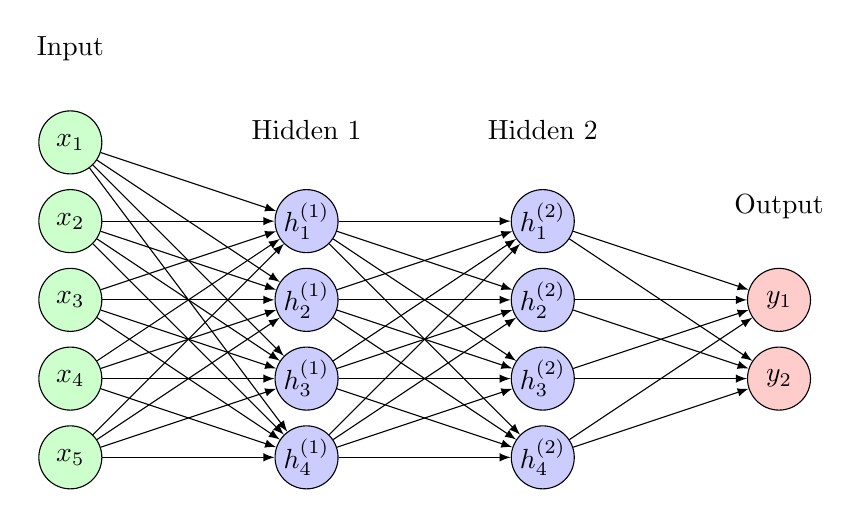
\begin{tikzpicture}[
        neuron/.style={circle, draw, minimum size=0.8cm, inner sep=0pt},
        input/.style={neuron, fill=green!20},
        hidden/.style={neuron, fill=blue!20},
        output/.style={neuron, fill=red!20},
        arrow/.style={->, >=latex}
    ]
        % Input Layer (5 Neuronen)
        \foreach \i in {1,...,5}
            \node[input] (I\i) at (0, -\i) {$x_{\i}$};

        % Hidden Layer 1 (4 Neuronen)
        \foreach \h in {1,...,4}
            \node[hidden] (H1\h) at (3, -\h - 1) {$h^{(1)}_{\h}$};

        % Hidden Layer 2 (4 Neuronen)
        \foreach \h in {1,...,4}
            \node[hidden] (H2\h) at (6, -\h - 1) {$h^{(2)}_{\h}$};

        % Output Layer (2 Neuronen)
        \foreach \o in {1,...,2}
            \node[output] (O\o) at (9, -\o - 2) {$y_{\o}$};
        
        % Labels
        \node[above=0.5cm] at (I1.north) {Input};
        \node[above=0.5cm] at (H11.north) {Hidden 1};
        \node[above=0.5cm] at (H21.north) {Hidden 2};
        \node[above=0.5cm] at (O1.north) {Output};

        % Verbindungen Input -> Hidden 1
        \foreach \i in {1,...,5}
            \foreach \h in {1,...,4}
                \draw[arrow] (I\i) -- (H1\h);

        % Verbindungen Hidden 1 -> Hidden 2
        \foreach \h in {1,...,4}
            \foreach \k in {1,...,4}
                \draw[arrow] (H1\h) -- (H2\k);

        % Verbindungen Hidden 2 -> Output
        \foreach \h in {1,...,4}
            \foreach \o in {1,...,2}
                \draw[arrow] (H2\h) -- (O\o);

    \end{tikzpicture}
    \caption{Schematische Darstellung der ursprünglichen, fully-connected Netzarchitektur.}
    \label{fig:nn_architektur_original}
\end{figure}

\begin{figure}[htbp]
    \centering
    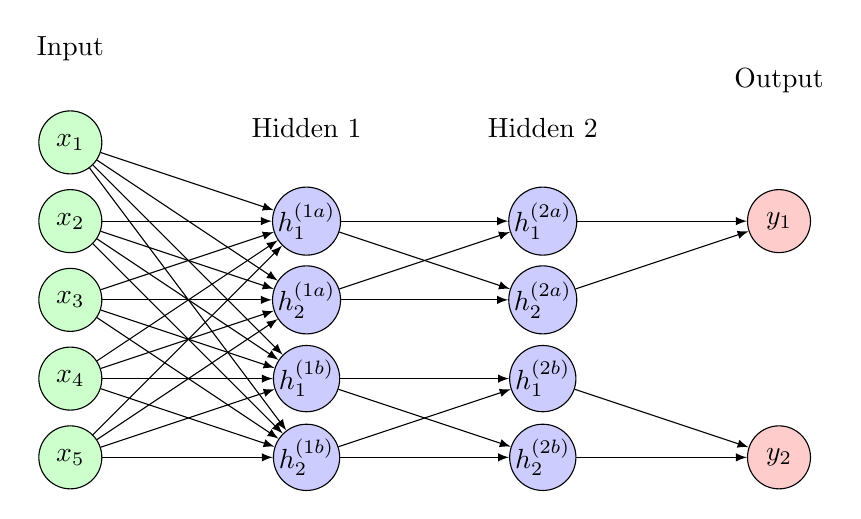
\begin{tikzpicture}[
        neuron/.style={circle, draw, minimum size=0.8cm, inner sep=0pt},
        input/.style={neuron, fill=green!20},
        hidden/.style={neuron, fill=blue!20},
        output/.style={neuron, fill=red!20},
        arrow/.style={->, >=latex}
    ]
        % Input Layer (5 Neuronen)
        \foreach \i in {1,...,5}
            \node[input] (I\i) at (0, -\i) {$x_{\i}$};

        % Hidden Layer 1 - Split (2 groups of 2)
        % Group A (Head 1)
        \foreach \h in {1,...,2}
            \node[hidden] (H1a\h) at (3, -\h - 1) {$h^{(1a)}_{\h}$};
        % Group B (Head 2)
        \foreach \h in {1,...,2}
            \node[hidden] (H1b\h) at (3, -\h - 3) {$h^{(1b)}_{\h}$};

        % Hidden Layer 2 - Split (2 groups of 2)
        % Group A (connected to y1)
        \foreach \h in {1,...,2}
            \node[hidden] (H2a\h) at (6, -\h - 1) {$h^{(2a)}_{\h}$};
        % Group B (connected to y2)
        \foreach \h in {1,...,2}
            \node[hidden] (H2b\h) at (6, -\h - 3) {$h^{(2b)}_{\h}$};

        % Output Layer (2 Neuronen)
        \node[output] (O1) at (9, -2) {$y_{1}$};
        \node[output] (O2) at (9, -5) {$y_{2}$};
        
        % Labels
        \node[above=0.5cm] at (I1.north) {Input};
        \node[above=0.5cm] at (H1a1.north) {Hidden 1};
        \node[above=0.5cm] at (H2a1.north) {Hidden 2};
        \node[above=0.5cm] at (9, -1) {Output};

        % Verbindungen Input -> Hidden 1 (A & B)
        \foreach \i in {1,...,5} {
            \foreach \k in {1,...,2} {
                \draw[arrow] (I\i) -- (H1a\k);
                \draw[arrow] (I\i) -- (H1b\k);
            }
        }

        % Verbindungen Hidden 1 A -> Hidden 2 A
        \foreach \h in {1,...,2}
            \foreach \k in {1,...,2}
                \draw[arrow] (H1a\h) -- (H2a\k);

        % Verbindungen Hidden 1 B -> Hidden 2 B
        \foreach \h in {1,...,2}
            \foreach \k in {1,...,2}
                \draw[arrow] (H1b\h) -- (H2b\k);

        % Verbindungen Hidden 2 A -> Output 1
        \foreach \h in {1,...,2}
            \draw[arrow] (H2a\h) -- (O1);

        % Verbindungen Hidden 2 B -> Output 2
        \foreach \h in {1,...,2}
            \draw[arrow] (H2b\h) -- (O2);

    \end{tikzpicture}
    \caption{Schematische Darstellung der Netzarchitektur mit vollständig getrennten Pfaden (Separate Heads) ab der Eingabeschicht.}
    \label{fig:nn_architektur_split}
\end{figure}

\begin{figure}[htbp]
    \centering
    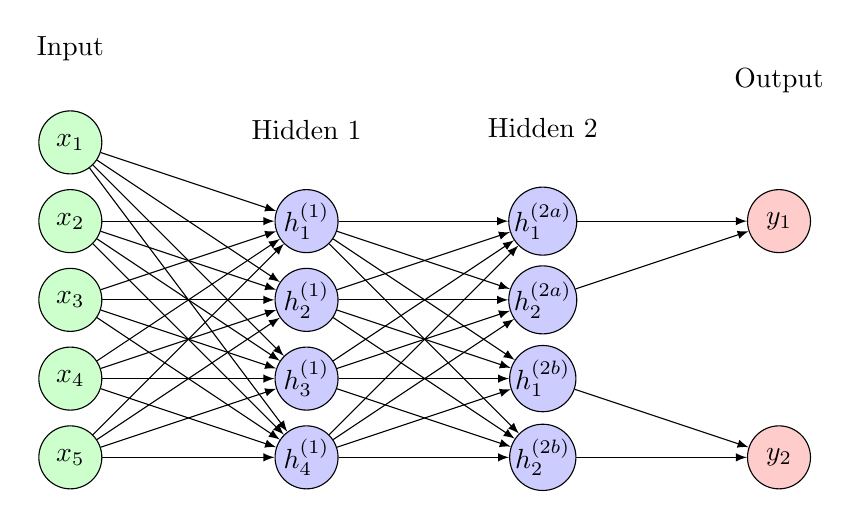
\begin{tikzpicture}[
        neuron/.style={circle, draw, minimum size=0.8cm, inner sep=0pt},
        input/.style={neuron, fill=green!20},
        hidden/.style={neuron, fill=blue!20},
        output/.style={neuron, fill=red!20},
        arrow/.style={->, >=latex}
    ]
        % Input Layer (5 Neuronen)
        \foreach \i in {1,...,5}
            \node[input] (I\i) at (0, -\i) {$x_{\i}$};

        % Hidden Layer 1 (4 Neuronen) - Shared
        \foreach \h in {1,...,4}
            \node[hidden] (H1\h) at (3, -\h - 1) {$h^{(1)}_{\h}$};

        % Hidden Layer 2 - Split (2 groups of 2)
        % Group A (Head 1)
        \foreach \h in {1,...,2}
            \node[hidden] (H2a\h) at (6, -\h - 1) {$h^{(2a)}_{\h}$};
        % Group B (Head 2)
        \foreach \h in {1,...,2}
            \node[hidden] (H2b\h) at (6, -\h - 3) {$h^{(2b)}_{\h}$};

        % Output Layer (2 Neuronen)
        \node[output] (O1) at (9, -2) {$y_{1}$};
        \node[output] (O2) at (9, -5) {$y_{2}$};
        
        % Labels
        \node[above=0.5cm] at (I1.north) {Input};
        \node[above=0.5cm] at (H11.north) {Hidden 1};
        \node[above=0.5cm] at (H2a1.north) {Hidden 2};
        \node[above=0.5cm] at (9, -1) {Output};

        % Verbindungen Input -> Hidden 1
        \foreach \i in {1,...,5}
            \foreach \h in {1,...,4}
                \draw[arrow] (I\i) -- (H1\h);

        % Verbindungen Hidden 1 -> Hidden 2 (A & B)
        \foreach \h in {1,...,4} {
            \foreach \k in {1,...,2} {
                \draw[arrow] (H1\h) -- (H2a\k);
                \draw[arrow] (H1\h) -- (H2b\k);
            }
        }

        % Verbindungen Hidden 2 A -> Output 1
        \foreach \h in {1,...,2}
            \draw[arrow] (H2a\h) -- (O1);

        % Verbindungen Hidden 2 B -> Output 2
        \foreach \h in {1,...,2}
            \draw[arrow] (H2b\h) -- (O2);

    \end{tikzpicture}
    \caption{Schematische Darstellung einer hybriden Netzarchitektur (Mischform). Die Pfade teilen sich zunächst gemeinsame Schichten (Shared Layers, hier Hidden 1), bevor sie sich trennen.}
    \label{fig:nn_architektur_hybrid}
\end{figure}

Die praktische Umsetzung dieser Architektur ist in Abbildung \ref{fig:nn_architektur_split} visualisiert, während Listing \ref{lst:branching_network} die zugehörige Implementierung zeigt. Im Gegensatz zur vollständig verbundenen Architektur in Abbildung \ref{fig:nn_architektur_original} werden hier bereits im ersten Hidden-Layer die Neuronen in funktional getrennte Gruppen unterteilt. Dieser Split zieht sich durch alle folgenden Schichten. Gruppe A verarbeitet Informationen exklusiv für den diskreten Aktionskopf ($y_1$), während Gruppe B ausschließlich den kontinuierlichen Ausgang ($y_2$) speist. Diese vollständige topologische Trennung verhindert sicher, dass der Optimierungsprozess für die Entscheidungskomponente die Repräsentationen für die Steuerungskomponente überschreibt.

